\chapter{Simple Modules}
\label{cha:simple-modules}
\index{module!simple}


\textit{Simple modules} are the active components in the model.
Simple modules are programmed in C++, using the {\opp} class
library. The following sections contain a short introduction
to discrete event simulation in general, explains how its concepts are
implemented in {\opp}, and gives an overview and practical advice
on how to design and code simple modules.



\section{Simulation concepts}

This section contains a very brief introduction into how Discrete
Event Simulation (DES) works, in order to introduce terms we'll use
when explaining {\opp} concepts\index{simulation!concepts} and
implementation. If you're familiar with DES\index{DES}, you can skip
the next few sections.




\subsection{Discrete Event Simulation}

A \textit{Discrete Event System} is a system where state changes
(events\index{events}) happen at discrete points of time, and events take zero time
to happen. It is assumed that nothing (i.e. nothing interesting)
happens between two consecutive events, that is, no state change takes
place in the system between the events (in contrast to
\textit{continuous} systems where state changes are continuous). Those
systems that can be viewed as Discrete Event Systems can be modeled
using Discrete Event Simulation\index{discrete event simulation}.
(Other systems can be modelled e.g. with continuous simulation models.)

For example, computer networks are usually viewed as discrete
event systems. Some of the events are:

\begin{itemize}
  \item{start of a packet transmission}
  \item{end of a packet transmission}
  \item{expiry of a retransmission timeout}
\end{itemize}


This implies that between two events such as \textit{start of a packet
transmission} and \textit{end of a packet transmission}, nothing
interesting happens. That is, the packet's state remains \textit{being
transmitted}. Note that the definition of ``interesting'' events and states always
depends on the intent and purposes of the person doing the modeling.
If we were interested in the transmission of individual bits, we would
have included something like \textit{start of bit transmission} and
\textit{end of bit transmission} among our events.


The time when events occur is often called \textit{event timestamp}
\index{event timestamp}; with {\opp} we'll say
\textit{arrival time}\index{arrival time} (because in the class
library, the word ``timestamp'' is reserved for a user-settable
attribute in the event class). Time within the model is often called
\textit{simulation time}\index{simulation time}, \textit{model time}
\index{model!time} or \textit{virtual time}\index{virtual time}
as opposed to real time\index{real time} or CPU time\index{CPU time}
or which refers to how long the simulation program has been running or
how much CPU time it has consumed.



\subsection{The event loop}

Discrete event simulations maintain the set of future
events\index{future events} in a data structure often called
FES\index{FES} (Future Event Set) or FEL\index{FEL} (Future Event List).
Such simulators usually work according to the following pseudocode:

\begin{Verbatim}[commandchars=\\\{\}]
\textit{initialize -- this includes building the model and}
              \textit{inserting initial events to FES}

\textit{while (FES not empty and simulation not yet complete)}
\textit{\{}
    \textit{retrieve first event from FES}
    \textit{t:= timestamp of this event}
    \textbf{\textit{process event}}
    \textit{(processing may insert new events in  FES or delete existing ones)}
\textit{\}}
\textit{finish simulation (write statistical results, etc.)}
\end{Verbatim}


The first, initialization step usually builds the data structures
representing the simulation model, calls any user-defined
initialization code, and inserts initial events\index{initial events}
into the FES to ensure that the simulation can start. Initialization
strategy can be quite different from one simulator to another.


The subsequent loop consumes events from the FES and processes
them. Events are processed in strict timestamp order in order
to maintain causality, that is, to ensure that no event may have
an effect on earlier events.

Processing an event involves calls to user-supplied code. For example,
using the computer network simulation example, processing a ``timeout
expired'' event may consist of re-sending a copy of the network
packet, updating the retry count, scheduling another ``timeout''
event, and so on. The user code may also remove events from the FES\index{FES},
for example when cancelling timeouts.

Simulation stops when there are no more events left (this happens
rarely in practice), or when it isn't necessary for the simulation
to run further because the model time or the CPU time has reached
a given limit, or because the statistics have reached the desired
accuracy. At this time, before the program exits, the simulation
programmer will typically want to record statistics into output
files.



\subsection{Simple modules in {\opp}}

In {\opp}, events occur inside simple modules\index{module!simple}.
Simple modules encapsulate C++ code that generate and react to events,
in other words, implement the behaviour of the model.

The user creates simple module types by subclassing the \cclass{cSimpleModule}
class, which is part of the {\opp} class library.
\cclass{cSimpleModule}, just as \cclass{cCompoundModule}, is derived
from a common base class, \cclass{cModule}.

\cclass{cSimpleModule}, although stuffed with simulation-related
functionality, doesn't do anything useful by itself -- you have
to redefine some virtual member functions to make it do useful work.


These member functions are the following:
\begin{itemize}
  \item{void \fname{initialize()}}
  \item{void \fname[handleMessage()]{handleMessage(cMessage *msg)}}
  \item{void \fname{activity()}}
  \item{void \fname{finish()}}
\end{itemize}

In the initialization step, {\opp} builds the network: it creates the
necessary simple\index{module!simple} and compound modules and
connects them according to the NED definitions. {\opp} also calls the
\fname{initialize()} functions of all modules.

The \fname{handleMessage()} and \fname{activity()} functions are
called during event processing. This means that the user will
implement the model's behavior in these functions.
\fname{handleMessage()} and \fname{activity()} implement
different event processing strategies: for each simple module, the user
has to redefine exactly one of these functions.

\fname{handleMessage()} is a method that is called
by the simulation kernel when the module receives a message.
\fname{activity()} is a coroutine-based\index{coroutine} solution
which implements the process interaction approach (coroutines are
non-preemptive (i.e. cooperative) threads). Generally, it is recommended
that you prefer \fname{handleMessage()} to \fname{activity()} --
mainly because \fname{activity()} doesn't scale well.
Later in this chapter we'll discuss both methods including their advantages
and disadvantages.

Modules written with \fname{activity()} and \fname{handleMessage()}
can be freely mixed within a simulation model.

The \fname{finish()} functions are called when the simulation
terminates successfully. The most typical use of \fname{finish()}
is the recording of statistics collected during simulation.



\subsection{Events in {\opp}}

{\opp} uses messages\index{message} to represent
events\index{events}. Each event is represented by an instance of the
\cclass{cMessage} class or one its subclasses; there is no separate
event class. Messages are sent from one module to another -- this
means that the place where the ``event will occur'' is the
\textit{message's destination module}, and the model time when the
event occurs is the \textit{arrival time}\index{arrival time} of the
message. Events like ``timeout expired'' are implemented with the
module sending a message to itself.

Simulation time in {\opp} is stored in the C++ type
\fvar{simtime\_t}, which is a typedef for \fvar{double}.

Events are consumed from the FES\index{FES} in arrival time order, to
maintain causality. More precisely, given two messages, the following
rules apply:
\begin{enumerate}
\item{the message with \textbf{earlier arrival time} is executed
    first.  If arrival times are equal,}
\item{the one with \textbf{smaller priority value} is executed first.
    If priorities are the same,}
\item{the one \textbf{scheduled or sent earlier} is executed first.}
\end{enumerate}

\textit{Priority}\index{message!priority} is a user-assigned integer
attribute of messages.

Storing simulation time in doubles may sometimes cause inconveniences.
Due to finite machine precision, two doubles calculated in two
different ways do not always compare equal even if they mathematically
should be. For example, addition is not an associative operation
when it comes to floating point calculations: $(x+y)+z != x+(y+z)$!
(See~\cite{Goldberg91what}).
This means that it is generally not a good idea to rely on
arrival times of two events being the same unless they are
calculated in exactly the same way.

One may suggest introducing a small \textit{simtime\_precision} parameter in
the simulation kernel that would force $t_{1}$ and $t_{2}$ to be regarded
equal if they are ``very close'' (if they differ
less than \textit{simtime\_precision}). This approach, however, would
be more likely to cause confusion than actually cure the problem.



\subsection{FES implementation}

The implementation of the FES\index{FES} is a crucial factor in the
performance of a discrete event simulator. In {\opp}, the FES is
implemented with \textit{binary heap}\index{binary heap}, the most
widely used data structure for this purpose. Heap is also the best
algorithm we know, although exotic data structures like
\textit{skiplist}\index{skiplist} may perform better than heap in some
cases. In case you're interested, the FES implementation is in the
\cclass{cMessageHeap} class, but as a simulation programmer you won't
ever need to care about it.





\section{Packet transmission modeling}
\label{ch:simple-modules:packet-transmission}

\subsection{Delay, bit error rate, data rate}

Connections can be assigned three parameters which facilitate
the modeling of communication networks, but can be useful for
other models too:
\begin{itemize}
  \item{propagation delay (sec)\index{channel!delay}}
  \item{bit error rate (errors/bit)\index{channel!error}}
  \item{data rate (bits/sec)\index{channel!datarate}}
\end{itemize}


Each of these parameters is optional. One can specify link parameters
individually for each connection, or define link types (also
called \textit{channel} \textit{types}) once and use them throughout the
whole model.

The \textit{propagation delay} is the amount of time the arrival of
the message is delayed by when it travels through the channel.
Propagation delay is specified in seconds.

The \textit{bit error rate} has influence on the transmission of messages
through the channel. The bit error rate (\textit{ber}) is the probability that
a bit is incorrectly transmitted. Thus, the probability that
a message of \textit{n} bits length is transferred without bit errors is:\\

$P_{no bit error} = (1 - ber)^length$

The message has an error flag which is set in case of transmission
errors.

The \textit{data rate} is specified in bits/second, and it is used
for transmission delay calculation. The sending time of the message
normally corresponds to the transmission of the first bit, and
the arrival time of the message corresponds to the reception
of the last bit (Fig. \ref{fig:ch-overview:message-transm}).

\begin{figure}[htbp]
\begin{center}
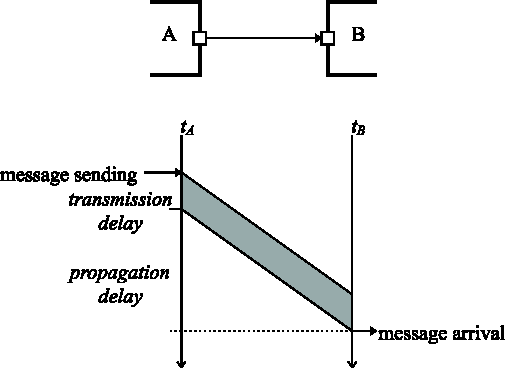
\includegraphics[width=4.301in, height=2.417in]{figures/usmanFig4}
\caption{Message transmission}
\label{fig:ch-overview:message-transm}
\end{center}
\end{figure}

The above model is not applicable for modeling some protocols like
Token Ring and FDDI where the stations repeat the bits of a frame that
arrives on the ring immediately, without waiting for the whole frame
to arrive; in other words, frames ``flow through'' the stations, being
delayed only a few bits. If you want to model such networks, the data
rate modeling feature of {\opp} cannot be used.

If a message travels along a route, through successive links and
compound modules, the model behaves as if each module waited until the
last bit of the message arrives and only start its transmission then
(Fig. \ref{fig:ch-overview:msg-multiple-ch}).

\begin{figure}[htbp]
\begin{center}
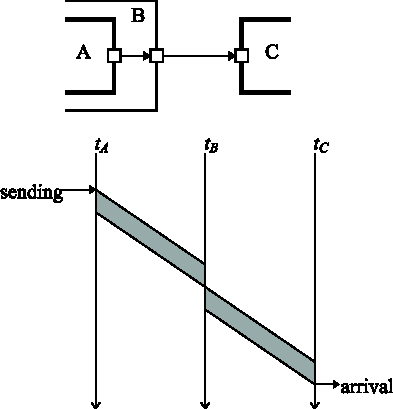
\includegraphics[width=3.330in, height=2.692in]{figures/usmanFig5}
\caption{Message sending over multiple channels}
\label{fig:ch-overview:msg-multiple-ch}
\end{center}
\end{figure}

Since the above effect is usually not the desired one, typically
you will want to assign data rate to only one connection in the
route.



\subsection{Multiple transmissions on links}


If data rate\index{data rate} is specified for a connection, a message
will have a certain nonzero transmission time\index{transmission
  time}, depending on its length.  This means that when a message is
sent out through an output gate, the message ``reserves'' the gate for
a given period (``it is being transmitted'').

\begin{figure}[htbp]
  \begin{center}
    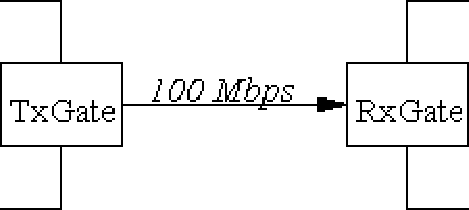
\includegraphics[width=2.315in, height=1.015in]{figures/usmanFig9}
    \caption{Connection with a data rate}
    \label{fig:ch-simple-modules:conn-w-data-rate}
  \end{center}
\end{figure}

While a message is under transmission, other messages have to wait
until the transmission finishes. You can still send messages
while the gate is busy, but the beginning of the modelled
message transmission will be delayed, just like the gate had
an internal queue for the messages waiting to be transmitted.

The {\opp} class library provides you with functions to check
whether a certain output gate is transmitting or to learn when
it finishes transmission.

If the connection with a data rate is not the immediate one connected
to the simple module's output gate but the second
one in the route, you have to check the second gate's busy
condition\index{gate!busy condition}.


\subsubsection{Implementation of message sending}


Message sending is implemented in the following way: the arrival
time\index{arrival time} and the bit error\index{bit error} flag of a
message are calculated at once, when the \fname{send()} (or similar)
function is invoked. That is, if the message travels through several
links until it reaches its destination, it is \textit{not} scheduled
individually for each link, but rather, every calculation is done
once, within the \fname{send()} call. This implementation was chosen
because of its run-time efficiency.

In the actual implementation of queuing the messages at busy gates and
modeling the transmission delay, messages do not actually queue up in
gates; gates do not have internal queues. Instead, as the time when
each gate will finish transmission is known at the time of sending the
message, the arrival time\index{arrival time} of the message can be
calculated in advance. Then the message will be stored in the event
queue (FES)\index{FES} until the simulation time advances to its
arrival time and it is retrieved by its destination module.

%
% TBD add pseudocode
%


\subsubsection{Consequence}


The implementation has the following consequence. If you change the
delay (or the bit error rate, or the data rate) of a link\index{link
  delay} during simulation, the modeling of messages sent ``just
before'' the parameter change will not be accurate. Namely, if link
parameters change while a message is ``under way'' in the model, that
message will not be affected by the parameter change, although it
should. However, all subsequent messages will be modelled correctly.
Similar for data rate: if a data rate changes during the simulation,
the change will affect only the messages that are \textit{sent} after
the change.

If it is important to model gates and channels with changing
properties, you can go two ways:
\begin{itemize}
  \item{write sender module such that they schedule events for when the
    gate finishes its current transmission and send then;}
  \item{alternatively, you can implement channels with
    simple modules (``active channels'').}
\end{itemize}


\subsubsection{The approach of some other simulators}


Note that some simulators (e.g. OPNET) assign \textit{packet queues}
to input gates (ports), and messages sent are buffered at the
destination module (or the remote end of the link) until received by
the destination module. With that approach, events and messages are
separate entities, that is, a \textit{send} operation includes placing
the message in the packet queue \textit{and} scheduling an event which
will signal the arrival of the packet. In some implementations, also
output gates have packet queues where packets wait until the channel
becomes free (available for transmission).

{\opp} gates\index{gate} don't have associated queues. The place
where the sent but not yet received messages are buffered is the
FES\index{FES}.  {\opp}'s approach is potentially faster
than the above mentioned solution because it doesn't have the
enqueue/dequeue overhead and also spares an event creation. The
drawback is, as mentioned above, that changes to channel parameters do
not take effect immediately.

In {\opp} one can implement \textit{point-to-point transmitter} modules
with packet queues if needed. For example, the INET Framework
follows this approach.




\section{Defining simple module types}

\subsection{Overview}

The C++ implementation of a simple\index{module!simple} module consists of:
\begin{itemize}
\item{declaration of the module class: your class subclassed from \cclass{cSimpleModule}
(either directly or indirectly)}
\item{a module type registration (\fmac{Define\_Module()} or
    \fmac{Define\_Module\_Like()} macro)}
\item{implementation of the module class}
\end{itemize}


For example, the C++ source for a Sliding Window Protocol implementation
might look like this:

\begin{verbatim}
// file: swp.cc
#include <omnetpp.h>

// module class declaration:
class SlidingWindowProtocol : public cSimpleModule
{
    Module_Class_Members(SlidingWindowProtocol,cSimpleModule,0)
    virtual void handleMessage(cMessage *msg);
};

// module type registration:
Define_Module( SlidingWindowProtocol );

// implementation of the module class:
void SlidingWindowProtocol::handleMessage(cMessage *msg)
{
   ...
}
\end{verbatim}

In order to be able to refer to this simple\index{module!simple} module type in NED
files, we should have an associated NED declaration which might
look like this:

\begin{Verbatim}[commandchars=\\\{\}]
// file: swp.ned
\textbf{simple} SlidingWindowProtocol
    \textbf{parameters}:
        windowSize: \textbf{numeric const};
    \textbf{gates}:
        \textbf{in:} fromNetw, fromHigherLayer;
        \textbf{out:} toNetw, toHigherLayer;
\textbf{endsimple}
\end{Verbatim}


\subsection{The module type registration}
\index{module!declaration}

The above example contained the following module type declaration:

\begin{verbatim}
Define_Module(SlidingWindowProtocol);
\end{verbatim}

This line tells {\opp} that you want to use the \ttt{SlidingWindowProtocol}
C++ class as a simple module type, and that it should look for an associated
NED simple module declaration with the same name (\ttt{simple SlidingWindowProtocol
... endsimple}) to determine what gates and parameters this module should have.

\fmac{Define\_Module()} should not be put into header files, because the compiler
generates code from it which should only appear in one \ttt{.cc} file.


\subsection{Several modules, single NED interface}

An alternative form of the module type registration, the \fmac{Define\_Module\_Like()}
macro takes two arguments and associates the class with a NED simple module
declaration of a different name. You can use this form when you have several
modules which share the same interface.

To support submodule types defined as parameters in
NED files (see section \ref{sec:ch-ned-lang:like}),
you can reuse an existing NED simple module definition
for several simple module types.

Suppose you have three different C++ module classes (\ttt{TokenRingMAC},
\ttt{EthernetMAC}, \ttt{FDDIMAC}) which have identical gates and parameters.
Then you can create a single NED declaration, \ttt{GenericMAC} for them
and write the following module type registrations in the C++ code:

\begin{verbatim}
Define_Module_Like(TokenRingMAC, GenericMAC);
Define_Module_Like(EthernetMAC, GenericMAC);
Define_Module_Like(FDDIMAC, GenericMAC);
\end{verbatim}

You won't be able to directly refer to the \ttt{TokenRingMAC},
\ttt{EthernetMAC}, \ttt{FDDIMAC} module types in your NED files,
because NED doesn't know about them (their names don't appear
in any NED file you could import), but you can use them wherever
a submodule type was defined as a parameter to the compound module:

\begin{verbatim}
module Host
    parameters:
        macType: string;
    submodules:
        mac: macType like GenericMAC;
                // if macType=="EthernetMAC" --> OK!
     ...
endmodule
\end{verbatim}

\begin{sloppypar}
The \ttt{macType} parameter should take the value \texttt{"TokenRingMAC"},
\texttt{"EthernetMAC"} or \texttt{"FDDIMAC"}, and a submodule of the appropriate
type will be created. The value for the parameter can even be given in
the ini file. This gives you a powerful tool to customize simulation
models (see also \textit{Topology templates}, Section
\ref{sec:ch-ned-lang:topology-templates}).
\end{sloppypar}




\subsection{The class declaration}

As mentioned before, simple\index{module!simple} module classes have
to be derived from \cclass{cSimpleModule} (either directly or
indirectly). In addition to overwriting some of the previously
mentioned four member functions (\fname{initialize()},
\fname{handleMessage()}, \fname{activity()}, \fname{finish()}), you
have to write a constructor\index{module!constructor} and some more
functions. Some of this task can be automated, so when writing the C++
class declaration, you have two choices:
\begin{enumerate}
\item{either use a macro which expands to the ``stock'' version of the
    functions}
\item{or write them yourself.}
\end{enumerate}

\subsubsection{Using macro to declare the constructor}

If you choose the first solution, you use the
\fmac{Module\_Class\_Members()} macro:

\begin{Verbatim}[commandchars=\\\{\}]
Module_Class_Members(\textit{classname}, \textit{baseclass}, \textit{stacksize});
\end{Verbatim}

The first two arguments are obvious (\textit{baseclass} is usually \cclass{cSimpleModule}),
but \textit{stacksize} needs some explanation. For simple modules implemented
with \ttt{handleMessage()} it should be zero, but if you use \fname{activity()},
the module code runs as a coroutine\index{coroutine}, so it will need a separate
stack of 16-32K. (This will be discussed in detail later.)


As an example, the class declaration

\begin{verbatim}
class SlidingWindowProtocol : public cSimpleModule
{
    Module_Class_Members(SlidingWindowProtocol,cSimpleModule,0)
    ...
};
\end{verbatim}

expands to something like this:

\begin{verbatim}
class SlidingWindowProtocol : public cSimpleModule
{
  public:
    SlidingWindowProtocol(const char *name, cModule *parent, unsigned stacksize=0) :
        cSimpleModule(name, parent, stacksize) {}
    ...
};
\end{verbatim}

\subsubsection{Expanded form of the constructor}

If you have data members in the class that you want to initialize in the
constructor, you cannot use the \ttt{Module\_Class\_Members()} macro.
Then you have to write the constructor yourself.

The constructor\index{module!constructor} should take the following
arguments (which you also have to pass further to the base class):

\begin{itemize}
  \item{\ttt{const char *name}, which is the name of the module}
  \item{\ttt{cModule *parentmodule}, pointer to the parent module}
  \item{\ttt{unsigned stacksize=\textit{stacksize}}, the coroutine stack size}
\end{itemize}

You should not change the number or types of the arguments taken
by the constructor, because it will be called by {\opp}-generated
code.

An example:

\begin{verbatim}
class TokenRingMAC : public cSimpleModule
{
  public:
    cQueue queue; // a data member
    TokenRingMAC(const char *name, cModule *parent, unsigned stacksize=0);
    ...
};

TokenRingMAC(const char *name, cModule *parent, unsigned stacksize) :
    cSimpleModule(name, parent, stacksize), queue("queue")
{
    // initialize data members
}
\end{verbatim}


\subsubsection{Stack size decides between handleMessage() and activity()}

\begin{itemize}
\item{if the specified stack size is zero, \fname{handleMessage()} will be used;}
\item{if it is greater than zero, \fname{activity()} will be used.}
\end{itemize}

If you make a mistake (e.g. you forget to set zero stack size
\index{zero stack size} for a \fname{handleMessage()}
simple module): the default versions of the
functions issue error messages telling you what is the problem.



\subsection{Using global variables}
\index{global variables}

If possible, avoid them global variables, including
static class members. There are several problems with them.
First, they are not reset to their initial values (to zero)
when you rebuild the simulation in Tkenv, or start another run
in Cmdenv. This may produce surprising results.

Second, they prevent you from running your simulation in parallel.
When using parallel simulation, each partition of your model
(may) run in a separate process, having its own copy of the
global variables. This is usually not what you want.




\section{Adding functionality to cSimpleModule}

This section discusses \cclass{cSimpleModule}'s four previously
mentioned member functions, intended to be redefined by the user:
\fname{initialize()}, \fname{handleMessage()}, \fname{activity()}
and \fname{finish()}.




\subsection{handleMessage()}

\subsubsection{Function called for each event}


The idea is that at each event\index{event} arrival we simply call a
user-defined function. This function,
\fname[handleMessage()]{handleMessage(cMessage *msg)} is a
virtual member function of \cclass{cSimpleModule} which does
nothing by default -- the user has to redefine it in subclasses
and add the message processing code.

The \fname{handleMessage()} function will be called for every message
that arrives at the module. The function should process the message
and return immediately after that. The simulation time is potentially
different in each call. No simulation time elapses within a call
to \fname{handleMessage()}.

The event loop inside the simulator handles both \fname{activity()}
and \fname{handleMessage()} simple modules, and it corresponds
to the following pseudocode:

\begin{Verbatim}[commandchars=\\\{\}]
\textit{while (FES not empty and simulation not yet complete)}
\{
    retrieve first event from FES
    t:= timestamp of this event
    m:= module containing this event
    if (m works with handleMessage())
        \textbf{m->handleMessage( event )}
    else // m works with activity()
        transferTo( m )
\}
\end{Verbatim}

Modules with \fname{handleMessage()} are NOT started automatically:
the simulation kernel creates starter messages\index{starter messages}
only for modules with \fname{activity()}. This means that you have to
schedule self-messages\index{self-message} from the
\fname{initialize()} function if you want a \fname{handleMessage()}
simple module to start working ``by itself'', without first receiving
a message from other modules.


\subsubsection{Programming with handleMessage()}


To use the \fname{handleMessage()} mechanism in a
simple module, you must specify \textit{zero
  stack size}\index{zero stack size} for the module. This is
important, because this tells {\opp} that you want to use
\fname{handleMessage()} and not \fname{activity()}.

Message/event related functions you can use in \fname{handleMessage()}:

\begin{itemize}
  \item{\fname{send()} family of functions -- to send messages to other modules}
  \item{\fname{scheduleAt()} -- to schedule an event (the module ``sends a message to itself'')}
  \item{\fname{cancelEvent()} -- to delete an event scheduled with \fname{scheduleAt()}}
\end{itemize}

You cannot use the \fname{receive()} family and
\fname{wait()} functions in \fname{handleMessage()}, because they are
coroutine-based by nature, as explained in the section about
\fname{activity()}.

You have to add data members to the module class for every piece
of information you want to preserve. This information cannot
be stored in local variables of \fname{handleMessage()} because they
are destroyed when the function returns. Also, they cannot be
stored in static variables in the function (or the class), because
they would be shared between all instances of the class.


Data members to be added to the module class will typically include
things like:

\begin{itemize}
  \item{state (e.g. IDLE/BUSY, CONN\_DOWN/CONN\_ALIVE/...)}
  \item{other variables which belong to the state of the module: retry
    counts, packet queues, etc.}
  \item{values retrieved/computed once and then stored: values of module
    parameters, gate indices, routing information, etc.}
  \item{pointers of message objects created once and then reused for
    timers, timeouts, etc.}
  \item{variables/objects for statistics collection}
\end{itemize}

You can initialize these variables from the \fname{initialize()}
function.  The constructor\index{module!constructor} is not a very good place
for this purpose, because it is called in the network setup phase when
the model is still under construction, so a lot of information you may
want to use is not yet available then.

Another task you have to do in \fname{initialize()} is to schedule
initial event(s)\index{events!initial} which trigger the first call(s)
to \fname{handleMessage()}.  After the first call,
\fname{handleMessage()} must take care to schedule further events for
itself so that the ``chain'' is not broken. Scheduling events is not
necessary if your module only has to react to messages coming from
other modules.

\fname{finish()} is used in the normal way: to record statistics information
accumulated in data members of the class at the end of the simulation.


\subsubsection{Application area}


\fname{handleMessage()} is in most cases a better choice than \fname{activity()}:

\begin{enumerate}
  \item{When you expect the module to be used in large simulations,
      involving several thousand modules. In such cases, the module stacks
      required by \fname{activity()} would simply consume too much memory.}
  \item{For modules which maintain little or no state information,
      such as packet sinks, \fname{handleMessage()} is more convenient to program.}
  \item{Other good candidates are modules with a large state space and
      many arbitrary state transition possibilities (i.e. where there
      are many possible subsequent states for any state). Such algorithms
      are difficult to program with \fname{activity()}, or the result is code
      which is better suited for \fname{handleMessage()} (see rule of thumb
      below). Most communication protocols are like this.}
\end{enumerate}


\subsubsection{Example 1: Protocol models}

Models of protocol layers in a communication network tend to have
a common structure on a high level because fundamentally they all have to react
to three types of events: to messages arriving from higher layer protocols
(or apps), to messages arriving from lower layer protocols (from the network),
and to various timers and timeouts (that is, self-messages).

This usually results in the following source code pattern:

\begin{verbatim}
class FooProtocol : public cSimpleModule
{
  protected:
    // state variables
    // ...

    virtual void processMsgFromHigherLayer(cMessage *packet);
    virtual void processMsgFromLowerLayer(FooPacket *packet);
    virtual void processTimer(cMessage *timer);

  public:
    Module_Class_Members(FooProtocol, cSimpleModule, 0);
    virtual void initialize();
    virtual void handleMessage(cMessage *msg);
};

// ...

void FooProtocol::handleMessage(cMessage *msg)
{
    if (msg->isSelfMessage())
        processTimer(msg);
    else if (msg->arrivedOn("fromNetw"))
        processMsgFromLowerLayer(check_and_cast<FooPacket *>(msg));
    else
        processMsgFromHigherLayer(msg);
}
\end{verbatim}

The functions \ttt{processMsgFromHigherLayer()}, \ttt{processMsgFromLowerLayer()}
and \ttt{processTimer()} are then usually split further: there are separate
methods to process separate packet types and separate timers.


\subsubsection{Example 2: Simple traffic generators and sinks}


The code for simple packet generators and sinks programmed with \fname{handleMessage()} might
be as simple as the following pseoudocode:

\begin{verbatim}
PacketGenerator::handleMessage(msg)
{
    create and send out a new packet;
    schedule msg again to trigger next call to handleMessage;
}

PacketSink::handleMessage(msg)
{
    delete msg;
}
\end{verbatim}

Note that \textit{PacketGenerator} will need to redefine \fname{initialize()}
to create \textit{m} and schedule the first event.

The following simple module generates packets with exponential
inter-arrival time. (Some details in the source haven't been
discussed yet, but the code is probably understandable nevertheless.)


\begin{Verbatim}[commandchars=\\\{\}]
class Generator : public cSimpleModule
\{
    Module_Class_Members(Generator,cSimpleModule,0)
                                // note zero stack size!
    virtual void initialize();
    virtual void handleMessage(cMessage *msg);
\};

Define_Module( Generator );

void Generator::initialize()
\{
    // schedule first sending
    scheduleAt(simTime(), new cMessage);
\}

void Generator::handleMessage(cMessage *msg)
\{
    // generate & send packet
    cMessage *pkt = new cMessage;
    send(pkt, "out");
    // schedule next call
    scheduleAt(simTime()+exponential(1.0), msg);
\}
\end{Verbatim}



\subsubsection{Example 3: Bursty traffic generator}


A bit more realistic example is to rewrite our Generator to create
packet bursts, each consisting of \ttt{burstLength} packets.

We add some data members to the class:
\begin{itemize}
\item{\ttt{burstLength} will store the parameter that specifies how many
    packets a burst must contain,}
\item{\ttt{burstCounter} will count in how many packets are left to be sent
    in the current burst.}
\end{itemize}

The code:

\begin{Verbatim}[commandchars=\\\{\}]
class BurstyGenerator : public cSimpleModule
\{
    Module_Class_Members(Generator,cSimpleModule,0)
    // note the zero stack size!
    int burstLength;
    int burstCounter;
    virtual void initialize();
    virtual void handleMessage(cMessage *msg);
\};

Define_Module( BurstyGenerator );
void BurstyGenerator::initialize()
\{
    // init parameters and state variables
    burstLength = par("burstLength");
    burstCounter = burstLength;
    // schedule first packet of first burst
    scheduleAt(simTime(), new cMessage);
\}

void BurstyGenerator::handleMessage(cMessage *msg)
\{
    // generate & send packet
    cMessage *pkt = new cMessage;
    send(pkt, "out");
    // if this was the last packet of the burst
    if (--burstCounter == 0)
    \{
        // schedule next burst
        burstCounter = burstLength;
        scheduleAt(simTime()+exponential(5.0), msg);
    \}
    else
    \{
        // schedule next sending within burst
        scheduleAt(simTime()+exponential(1.0), msg);
    \}
\}
\end{Verbatim}



\subsubsection{Pros and Cons of using \fname{handleMessage()}}


Pros:
\begin{itemize}
  \item{consumes less memory: no separate stack needed for simple modules}
  \item{fast: function call is faster than switching between coroutines\index{coroutine}}
\end{itemize}

Cons:
\begin{itemize}
  \item{local variables cannot be used to store state information}
  \item{need to redefine \fname{initialize()}}
\end{itemize}

Usually, \fname{handleMessage()} should be preferred to \fname{activity()}.


\subsubsection{Other simulators}


Many simulation packages use a similar approach, often topped with
something like a state machine\index{finite state machine}
(FSM\index{FSM}) which hides the underlying function calls. Such
systems are:
\begin{itemize}
  \item{OPNET$^TM$ which uses FSM's designed using a graphical editor;}
  \item{NetSim++ clones OPNET's approach;}
  \item{SMURPH (University of Alberta) defines a (somewhat eclectic)
      language to describe FSMs, and uses a precompiler to turn it
      into C++ code;}
  \item{Ptolemy (UC Berkeley) uses a similar method.}
\end{itemize}

{\opp}'s FSM\index{FSM} support is described in the next section.



\subsection{activity()}

\subsubsection{Process-style description}

With \fname{activity()}, you can code the simple
module much like you would code an operating system process or a
thread. You can wait for an incoming message (event) at any point of
the code, you can suspend the execution for some time (model time!),
etc. When the \fname{activity()} function exits, the module is
terminated.  (The simulation can continue if there are other modules
which can run.)


The most important functions you can use in \fname{activity()} are
(they will be discussed in detail later):
\begin{itemize}
\item{\fname{receive()} -- to receive messages (events)}
\item{\fname{wait()} -- to suspend execution\index{suspend execution}
    for some time (model time)}
\item{\fname{send()} family of functions -- to send messages to other
    modules}
\item{\fname{scheduleAt()} -- to schedule an event (the module ``sends
    a message to itself'')}
\item{\fname{cancelEvent()} -- to delete an event scheduled with
    scheduleAt()}
\item{\fname{end()} -- to finish execution of this module (same as
    exiting the \fname{activity()} function)}
\end{itemize}

The \fname{activity()} function normally contains an infinite loop,
with at least a \fname{wait()} or \fname{receive()} call in its body.



\subsubsection{Application area}

Generally you should prefer \ttt{handleMessage()} to \ttt{activity()}.
The main problem with \ttt{activity()} is that it doesn't scale because
every module needs a separate coroutine stack. It has also been observed
that \ttt{activity()} does not encourage a good programming style.

However, there is one scenario where \ttt{activity()}'s process-style
description is convenient: when the process has many
states but transitions are very limited, ie. from any state the
process can only go to one or two other states.  For example, this is
the case when programming a network application which uses a single
network connection.  The pseudocode of the application which talks to
a transport layer protocol might look like this:

\begin{Verbatim}[commandchars=\\\{\}]
\textit{activity()}
\{
    while(true)
    \{
        open connection by sending OPEN command to transport layer
        receive reply from transport layer
        if (open not successful)
        \{
            wait(some time)
            continue // loop back to while()
        \}

        while(there's more to do)
        \{
            send data on network connection
            if (connection broken)
            \{
                continue outer loop // loop back to outer while()
            \}
            wait(some time)
            receive data on network connection
            if (connection broken)
            \{
                continue outer loop // loop back to outer while()
            \}
            wait(some time)
        \}
        close connection by sending CLOSE command to transport layer
        if (close not successful)
        \{
            // handle error
        \}
        wait(some time)
    \}
\}
\end{Verbatim}

If you have to handle several connections simultaneously, you may
dynamically create as instances of the simple module above.
Dynamic module creation will be discussed later.

There are situations when you certainly \textit{do not want} to use \fname{activity()}.
If your \fname{activity()} function contains no \fname{wait()} and it has
only one \fname{receive()} call at the top of an infinite loop,
there's no point in using \ttt{activity()} and the code should be written
with \ttt{handleMessage()}.
The body of the infinite loop would then become the body to \fname{handleMessage()},
state variables inside \fname{activity()} would become data members in
the module class, and you'd initialize them in \fname{initialize()}.

Example:

\begin{verbatim}
void Sink::activity()
{
    while(true)
    {
        msg = receive();
        delete msg;
    }
}
\end{verbatim}

should rather be programmed as:

\begin{verbatim}
void Sink::handleMessage(cMessage *msg)
{
    delete msg;
}
\end{verbatim}



\subsubsection{Activity() is run as a coroutine}


\fname[activity()]{Activity()} is run in a coroutine\index{coroutine}.
Coroutines are a sort of threads\index{threads} which are scheduled
non-preemptively (this is also called cooperative
multitasking\index{multitasking!cooperative}). From one coroutine you
can switch to another coroutine by a
\fname[transferTo()]{transferTo(otherCoroutine)} call. Then this
coroutine is suspended and \textit{otherCoroutine} will run. Later,
when \textit{otherCoroutine} does a
\fname[transferTo()]{transferTo(firstCoroutine)} call, execution of
the first coroutine will resume from the point of the
\fname[transferTo()]{transferTo(otherCoroutine)} call.  The full state
of the coroutine, including local variables are preserved while the
thread of execution is in another coroutines.  This implies that each
coroutine must have an own processor stack\index{stack}, and
\fname{transferTo()} involves a switch from one processor stack to
another.


Coroutines\index{coroutine} are at the heart of {\opp}, and the
simulation programmer doesn't ever need to call \fname{transferTo()}
or other functions in the coroutine library, nor does he need to care
about the coroutine library implementation. But it is important to
understand how the event loop found in discrete event simulators works
with coroutines.


When using coroutines, the event loop\index{event loop} looks like
this (simplified):


\begin{Verbatim}[commandchars=\\\{\}]
\textit{while (FES not empty and simulation not yet complete)}
\{
    retrieve first event from FES
    t:= timestamp of this event
    \textbf{transferTo(module containing the event)}
\}
\end{Verbatim}



That is, when the module has an event\index{event}, the simulation
kernel transfers the control to the module's coroutine. It is expected
that when the module ``decides it has finished the processing of the
event'', it will transfer the control back to the simulation kernel by
a \fname[transferTo()]{transferTo(main)} call. Initially,
simple\index{module!simple} modules using \fname{activity()} are
``booted'' by events (\textit{''starter messages''}\index{starter messages})
inserted into the FES by the simulation kernel before the
start of the simulation.


How does the coroutine know it has ``finished processing the event''?
The answer: \textit{when it requests another event}.  The functions
which request events from the simulation kernel are the
\fname{receive()} and \fname{wait()}, so their
implementations contain a \fname[transferTo()]{transferTo(main)} call
somewhere.


Their pseudocode, as implemented in {\opp}:


\begin{Verbatim}[commandchars=\\\{\}]
receive()
\{
    transferTo(main)
    retrieve current event
    return the event // remember: events = messages
\}

wait()
\{
    create event e
    schedule it at (current sim. time + wait interval)
    transferTo(main)
    retrieve current event
    if (current event is not e) \{
        error
    \}
    delete e  // note: actual impl. reuses events
    return
\}
\end{Verbatim}



Thus, the \fname{receive()} and \fname{wait()} calls are
special points in the \fname{activity()} function, because that's
where:

\begin{itemize}
  \item{simulation time elapses in the module, and}
  \item{other modules get a chance to execute.}
\end{itemize}


\subsubsection{Starter messages}


Modules written with \fname{activity()} need starter
messages\index{starter messages} to ``boot''.  These starter messages
are inserted into the FES\index{FES} automatically by {\opp} at the
beginning of the simulation, even before the \fname{initialize()}
functions are called.


\subsubsection{Coroutine stack size}


All the simulation programmer needs to care about coroutines is to
choose the processor stack size\index{coroutine!stack size} for them.
This cannot be automated.

16 or 32 kbytes is usually a good choice, but you may need more if the
module uses recursive functions or has local variables which occupy a
lot of stack space. {\opp} has a built-mechanism that will usually
detect if the module stack is too small and
overflows\index{stack!overflow}. {\opp} can also tell you how much
stack space a module actually uses\index{stack!usage}, so you can find
it out if you overestimated the stack needs.


\subsubsection{initialize() and finish() with activity()}


Because local variables of \fname{activity()} are preserved across
events, you can store everything (state information, packet buffers,
etc.) in them. Local variables can be initialized at the top of the
\fname{activity()} function, so there isn't much need to use
\fname{initialize()}.


However, you need \fname{finish()} if you want to write statistics at
the end of the simulation. And because \fname{finish()} cannot access
the local variables of \fname{activity()}, you have to put the variables
and objects that contain the statistics into the module class.
You still don't need \fname{initialize()} because class members can also
be initialized at the top of \fname{activity()}.


Thus, a typical setup looks like this pseudocode:


\begin{Verbatim}[commandchars=\\\{\}]
\textit{class MySimpleModule...}
\{
    ...
    variables for statistics collection
    activity();
    finish();
\};

MySimpleModule::activity()
\{
    declare local vars and initialize them
    initialize statistics collection variables

    while(true)
    \{
        ...
    \}
\}

MySimpleModule::finish()
\{
    record statistics into file
\}
\end{Verbatim}


\subsubsection{Pros and Cons of using \fname{activity()}}


Pro:
\begin{itemize}
   \item{\fname{initialize()} not needed, state can be stored in local
       variables of \fname{activity()}}
   \item{process-style description is a natural programming model in some cases}
\end{itemize}

Con:
\begin{itemize}
   \item{limited scalability: coroutine stacks can unacceptably increase the
       memory requirements of the simulation program if you have several
       thousands or ten thousands of simple modules;}
   \item{run-time overhead: switching between coroutines is somewhat slower
       than a simple function call}
   \item{does not enforce a good programming style: using \ttt{activity()}
       tends to lead to unreliable, spaghetti code}
\end{itemize}

In most cases, cons outweigh pros and it is a better idea to use
\ttt{handleMessage()} instead.


\subsubsection{Other simulators}


Coroutines are used by a number of other simulation packages:
\begin{itemize}
\item{All simulation software which inherit from SIMULA (e.g. C++SIM)
    are based on coroutines, although all in all the programming
    model is quite different.}
\item{The simulation/parallel programming language Maisie and its successor
    PARSEC (from UCLA) also use coroutines (although implemented
    on with ``normal'' preemptive threads). The philosophy
    is quite similar to {\opp}. PARSEC, being ``just''
    a programming language, has a more elegant syntax but much less
    features than {\opp}.}
\item{Many Java-based simulation libraries are based on Java
    threads.}
\end{itemize}




\subsection{initialize() and finish()}

\subsubsection{Purpose}


\fname{initialize()} -- to provide place for any user setup code

\fname{finish()} -- to provide place where the user can record statistics
after the simulation has completed


\subsubsection{When and how they are called}


The \fname{initialize()} functions of the modules are invoked
\textit{before} the first event is processed, but \textit{after} the
initial events (starter messages\index{starter messages}) have been
placed into the FES by the simulation kernel.


Both simple and compound modules have \fname{initialize()} functions.
A compound module has its \fname{initialize()} function called
\textit{before} all its submodules have.


The \fname{finish()} functions are called when the event
loop\index{event loop} has terminated, and only if it terminated
normally (i.e. not with a runtime error).  The calling order is the
reverse as with \fname{initialize()}: first submodules, then the
containing compound module. (The bottom line is that at the moment
there's no ``official'' possibility to redefine \fname{initialize()}
and \fname{finish()} for compound modules; the unofficial way is to
write into the nedtool-generated C++ code. Future versions of {\opp} will
support adding these functions to compound modules.)

This is summarized in the following pseudocode (although you
won't find this code ``as is'' in the simulation
kernel sources):


\begin{Verbatim}[commandchars=\\\{\}]
\textit{perform simulation run:}
    build network
      (i.e. the system module and its submodules recursively)
    insert starter messages for all submodules using activity()
    do callInitialize() on system module
        \textit{enter event loop // (described earlier)}
    if (event loop terminated normally) // i.e. no errors
        do callFinish() on system module
    clean up

callInitialize()
\{
    call to user-defined initialize() function
    if (module is compound)
        for (each submodule)
            do callInitialize() on submodule
\}

callFinish()
\{
    if (module is compound)
        for (each submodule)
            do callFinish() on submodule
    call to user-defined finish() function
\}
\end{Verbatim}



\subsubsection{initialize() vs. constructor}


Usually you should not put simulation-related code into the
simple module constructor\index{module!constructor}. For
example, modules often need to investigate their surroundings (maybe
the whole network) at the beginning of the simulation and save the
collected info into internal tables.  Code like that cannot be placed
into the constructor since the network is still being set up when the
constructor is called.


\subsubsection{finish() vs. destructor}


Keep in mind that \fname{finish()} is not always called, so it isn't a
good place for cleanup code which should run every time the module is
deleted. \fname{finish()} is only a good place for writing statistics,
result post-processing and other stuff which are to run only on
successful completion.

Cleanup code should go into the destructor\index{module!destructor}. But in
fact, you almost never need to write a destructor because {\opp}
keeps track of objects you create and disposes of them automatically
(sort of automatic garbage collection). However it cannot track
objects not derived from \cclass{cObject}, so they may
need to be deleted manually from the destructor. Garbage collection
is discussed in more detail in section \ref{sec:ch-sim-lib:garbage-collection}.



\subsubsection{Multi-stage initialization}


In simulation models, when one-stage
initialization\index{initialization} provided by \fname{initialize()}
is not sufficient, one can use multi-stage
initialization\index{initialization!multi-stage}.  Modules have two
functions which can be redefined by the user:

\begin{verbatim}
void initialize(int stage);
int numInitStages() const;
\end{verbatim}

At the beginning of the simulation, \fname[initialize]{initialize(0)}
is called for \textit{all} modules, then \fname[initialize()]{initialize(1)},
\fname[initialize()]{initialize(2)}, etc. You can think of it like
initialization takes place in several ``waves''. For each module,
\fname{numInitStages()} must be redefined to return the number of init
stages required, e.g. for a two-stage init, \fname{numInitStages()}
should return 2, and \fname{initialize(int stage)} must be implemented to
handle the \textit{stage=0} and \textit{stage=1} cases.
  \footnote{Note \ttt{const} in the \ttt{numInitStages()} declaration.
  If you forget it, by C++ rules you create a \textit{different} function
  instead of redefining the existing one in the base class, thus the
  existing one will remain in effect and return 1.}

The \fname{callInitialize()} function performs the full multi-stage initialization
for that module and all its submodules.

If you do not redefine the multi-stage initialization functions, the
default behavior is single-stage initialization: the default
\fname{numInitStages()} returns 1, and the default \fname[initialize]{initialize(int
stage)} simply calls \fname{initialize()}.


\subsubsection{``End-of-Simulation'' event}


The task of \fname{finish()} is solved in many simulators (e.g. OPNET)
by introducing a special
\textit{end-of-simulation}\index{end-of-simulation} event. This is not
a very good practice because the simulation programmer has to code the
models (often represented as FSMs) so that they can \textit{always} properly
respond to end-of-simulation events, in whichever state they are. This
often makes program code unnecessarily complicated.

This fact is also evidenced in the design of the PARSEC\index{PARSEC}
simulation language (UCLA). Its predecessor Maisie used
end-of-simulation events, but -- as documented in the PARSEC manual --
this has led to awkward programming in many cases, so for PARSEC
end-of-simulation events were dropped in favour of \fname{finish()}
(called \fname{finalize()} in PARSEC).



\subsection{Reusing module code via subclassing}

It is often needed to have several variants of a simple module.
A good design strategy is to create a simple module class with
the common functionality, then subclass from it to create the
specific simple module types.

% FIXME use QueueBase example!

An example:

\begin{verbatim}
class ModifiedTransportProtocol : public TransportProtocol
{
  public:
    Module_Class_Members(ModifiedTransportProtocol, TransportProtocol,0)
    virtual void recalculateTimeout();
};

Define_Module( ModifiedTransportProtocol );

void ModifiedTransportProtocol::recalculateTimeout()
{
    //...
}
\end{verbatim}


\section{Finite State Machines in {\opp}}

\subsubsection{Overview}


Finite State Machines\index{finite state machine} (FSMs)\index{FSM}
can make life with \fname{handleMessage()} easier. {\opp} provides a
class and a set of macros to build FSMs. {\opp}'s FSMs work very much
like OPNET's or SDL's.


The key points are:
\begin{itemize}
\item{There are two kinds of states:
    \textit{transient}\index{transient states} and
    \textit{steady}\index{steady states}. At each event (that is, at
    each call to \fname{handleMessage()}), the FSM transitions out of
    the current (\textit{steady}) state, undergoes a series of state
    changes (runs through a number of \textit{transient} states), and
    finally arrives at another \textit{steady} state. Thus between two
    events, the system is always in one of the steady states.
    Transient states are therefore not really a must -- they exist
    only to group actions to be taken during a transition in a
    convenient way.}
\item{You can assign program code to entering and leaving a state
    (known as entry/exit code)\index{entry code}\index{exit code}.
    Staying in the same state is handled as leaving and re-entering
    the state.}
\item{Entry code should not modify the state (this is verified by
    {\opp}).  State changes (transitions) must be put into the exit
    code.}
\end{itemize}

{\opp}'s FSMs \textit{can} be nested\index{FSM!nested}. This means
that any state (or rather, its entry or exit code) may contain a
further full-fledged \fmac{FSM\_Switch()} (see below). This allows you
to introduce sub-states and thereby bring some structure into the
state space if it would become too large.


\subsubsection{The FSM API}


FSM state is stored in an object of type \cclass{cFSM}. The possible states
are defined by an enum; the enum is also a place to tell which
state is transient and which is steady. In the following example, SLEEP
and ACTIVE are steady states and SEND is transient (the numbers
in parens must be unique within the state type and they are used
for constructing the numeric IDs for the states):

\begin{verbatim}
enum {
  INIT = 0,
  SLEEP = FSM_Steady(1),
  ACTIVE = FSM_Steady(2),
  SEND = FSM_Transient(1),
};
\end{verbatim}



The actual FSM is embedded in a switch-like statement,
\fmac{FSM\_Switch()}, where you have cases for entering and leaving
each state:


\begin{Verbatim}[commandchars=\\\{\}]
FSM_Switch(fsm)
\{
  case FSM_Exit(\textit{state1}):
    //...
  break;
  case FSM_Enter(\textit{state1}):
    //...
  break;
  case FSM_Exit(\textit{state2}):
    //...
  break;
  case FSM_Enter(\textit{state2}):
    //...
  break;
    //...
\};
\end{Verbatim}


State transitions\index{state transition} are done via calls to
\fmac{FSM\_Goto()}, which simply stores the new state in the
\cclass{cFSM} object:

\begin{Verbatim}[commandchars=\\\{\}]
FSM_Goto(fsm,\textit{newState});
\end{Verbatim}

The FSM starts from the state with the numeric code 0; this state
is conventionally named INIT.


\subsubsection{Debugging FSMs}

FSMs can log their state transitions \ttt{ev}\index{ev},
with the output looking like this:

\begin{verbatim}
...
FSM GenState: leaving state SLEEP
FSM GenState: entering state ACTIVE
...
FSM GenState: leaving state ACTIVE
FSM GenState: entering state SEND
FSM GenState: leaving state SEND
FSM GenState: entering state ACTIVE
...
FSM GenState: leaving state ACTIVE
FSM GenState: entering state SLEEP
...
\end{verbatim}

To enable the above output, you have to \ttt{\#define FSM\_DEBUG}\index{FSM\_DEBUG}
before including \ttt{omnetpp.h}.

\begin{Verbatim}[commandchars=\\\{\}]
#define FSM_DEBUG    // enables debug output from FSMs
#include <omnetpp.h>
\end{Verbatim}

The actual logging is done via the \fmac{FSM\_Print()} macro.
It is currently defined as follows, but you can change the
output format by undefining \ttt{FSM\_Print()} after including
\ttt{omnetpp.ini} and providing a new definition instead.

\begin{verbatim}
#define FSM_Print(fsm,exiting)
  (ev << "FSM " << (fsm).name()
      << ((exiting) ? ": leaving state " : ": entering state ")
      << (fsm).stateName() << endl)
\end{verbatim}


\subsubsection{Implementation}


The \fmac{FSM\_Switch()} is a macro. It expands to a \fname{switch()}
statement embedded in a \fname{for()} loop which repeats until the
FSM\index{FSM} reaches a steady state. (The actual code is rather
ugly, but if you're dying to see it, it's in \texttt{cfsm.h}.)

Infinite loops are avoided by counting state transitions: if
an FSM goes through 64 transitions without reaching a steady
state, the simulation will terminate with an error message.


\subsubsection{An example}


Let us write another flavour of a bursty generator. It has two
states, SLEEP and ACTIVE. In the SLEEP state, the module does
nothing. In the ACTIVE state, it sends messages with a given
inter-arrival time. The code was taken from the Fifo2 sample
simulation.


\begin{Verbatim}[commandchars=\\\{\}]
#define FSM_DEBUG
#include <omnetpp.h>

class BurstyGenerator : public cSimpleModule
\{
 public:
  Module_Class_Members(BurstyGenerator,cSimpleModule,0);

  // parameters
  double sleepTimeMean;
  double burstTimeMean;
  double sendIATime;
  cPar *msgLength;

  // FSM and its states
  cFSM fsm;
  enum \{
    INIT = 0,
    SLEEP = FSM_Steady(1),
    ACTIVE = FSM_Steady(2),
    SEND = FSM_Transient(1),
  \};

  // variables used
  int i;
  cMessage *startStopBurst;
  cMessage *sendMessage;

  // the virtual functions
  virtual void initialize();
  virtual void handleMessage(cMessage *msg);
\};

Define_Module( BurstyGenerator );

void BurstyGenerator::initialize()
\{
  fsm.setName("fsm");
  sleepTimeMean = par("sleepTimeMean");
  burstTimeMean = par("burstTimeMean");
  sendIATime = par("sendIATime");
  msgLength = &par("msgLength");
  i = 0;
  WATCH(i); // always put watches in initialize()
  startStopBurst = new cMessage("startStopBurst");
  sendMessage = new cMessage("sendMessage");
  scheduleAt(0.0,startStopBurst);
\}

void BurstyGenerator::handleMessage(cMessage *msg)
\{
  FSM_Switch(fsm)
 \{
    case FSM_Exit(INIT):
      // transition to SLEEP state
      FSM_Goto(fsm,SLEEP);
      break;
    case FSM_Enter(SLEEP):
      // schedule end of sleep period (start of next burst)
      scheduleAt(simTime()+exponential(sleepTimeMean),
                 startStopBurst);
    break;
    case FSM_Exit(SLEEP):
      // schedule end of this burst
      scheduleAt(simTime()+exponential(burstTimeMean),
                 startStopBurst);
      // transition to ACTIVE state:
      if (msg!=startStopBurst) \{
        error("invalid event in state ACTIVE");
      \}
      FSM_Goto(fsm,ACTIVE);
      break;
    case FSM_Enter(ACTIVE):
      // schedule next sending
      scheduleAt(simTime()+exponential(sendIATime), sendMessage);
    break;
    case FSM_Exit(ACTIVE):
      // transition to either SEND or SLEEP
      if (msg==sendMessage) \{
        FSM_Goto(fsm,SEND);
      \} else if (msg==startStopBurst) \{
        cancelEvent(sendMessage);
        FSM_Goto(fsm,SLEEP);
      \} else \{
        error("invalid event in state ACTIVE");
      \}
      break;
    case FSM_Exit(SEND):
    \{
      // generate and send out job
      char msgname[32];
      sprintf( msgname, "job-%d", ++i);
      ev << "Generating " << msgname << endl;
      cMessage *job = new cMessage(msgname);
      job->setLength( (long) *msgLength );
      job->setTimestamp();
      send( job, "out" );
      // return to ACTIVE
      FSM_Goto(fsm,ACTIVE);
      break;
    \}
  \}
\}
\end{Verbatim}





\section{Sending and receiving messages}
\label{ch:simple-modules:sending-and-receiving}

On an abstract level, an {\opp} simulation model is a set of
simple modules that communicate with each other via message passing.
The essence of simple modules is that they create, send, receive,
store, modify, schedule and destroy messages -- everything else
is supposed to facilitate this task, and collect statistics
about what was going on.

Messages in {\opp} are instances of the \ttt{cMessage} class or
one of its subclasses. Message objects are created using the C++
\ttt{new} operator and destroyed using the \ttt{delete} operator
when they are no longer needed. During their lifetimes,
messages travel between modules via gates and connections
(or are sent directly, bypassing the connections), or
they are scheduled by and delivered to modules,
representing internal events of that module.

Messages are described in detail in chapter \ref{cha:messages}.
At this point, all we need to know about them is that they are
referred to as \ttt{cMessage *} pointers. Message objects
can be given descriptive names (a \ttt{const char *} string)
that often helps in debugging the simulation. The message
name string can be specified in the constructor, so it
should not surprise you if you see something like
\ttt{new cMessage("token")} in the examples below.



\subsection{Sending messages}

Once created, a message object can be sent through an
output gate\index{output!gate} using one of the following functions:

\begin{verbatim}
send(cMessage *msg, const char *gateName, int index=0);
send(cMessage *msg, int gateId);
send(cMessage *msg, cGate *gate);
\end{verbatim}

In the first function, the argument \ttt{gateName} is the name of
the gate the message has to be sent through. If this gate is
a vector gate, \ttt{index} determines though which particular output
gate this has to be done; otherwise, the \ttt{index} argument is not
needed.

The second and third functions use the gate Id and the pointer to the gate
object. They are faster than the third one because they don't have to
search through the gate array.

Examples:

\begin{verbatim}
send(msg, "outGate");
send(msg, "outGates", i); // send via outGates[i]
\end{verbatim}

The following code example creates and sends messages
every 5 simulated seconds:

\begin{verbatim}
int outGateId = findGate("outGate");
while(true)
{
  send(new cMessage("packet"), outGateId);
  wait(5);
}
\end{verbatim}


\subsubsection{Modeling packet transmissions}

If you're sending messages over a link that has (nonzero) data rate,
it is modeled in the way that has been described earlier in this
manual, in section \ref{ch:simple-modules:packet-transmission}.

If you want to have full control over the transmission process,
you'll probably need the \fname{isBusy()} and \fname{transmissionFinishes()}
member functions of \cclass{cGate}. They are described in section
\ref{ch:simple-modules:cgate-transmission-state}.



\subsection{Broadcasts and retransmissions}

When you implement broadcasts or retransmissions, two frequently
occurring tasks in protocol simulation, you might feel tempted
to use the same message in multiple \fname{send()} operations.
Do not do it -- you cannot send the same message object multiple times.
The solution in such cases is duplicating the message.

\subsubsection{Broadcasting messages}

In your model, you may need to broadcast a message to several destinations.
Broadcast can be implemented in a simple module by sending out copies
of the same message, for example on every gate of a gate vector.
As described above, you cannot use the same message pointer for
in all \fname{send()} calls -- what you have to do instead is
create copies (duplicates) of the message object and send them.

Example:

\begin{verbatim}
for (int i=0; i<n; i++)
{
    cMessage *copy = (cMessage *) msg->dup();
    send(copy, "out", i);
}
delete msg;
\end{verbatim}

You might have noticed that copying the message for the last gate is
redundant (we could send out the original message),
so it can be optimized out like this:

\begin{verbatim}
for (int i=0; i<n-1; i++)   // note n-1 instead of n
{
    cMessage *copy = (cMessage *) msg->dup();
    send(copy, "out", i);
}
send(msg, "out", n-1);  // send original on last gate
\end{verbatim}


\subsubsection{Retransmissions}

Many communication protocols involve retransmissions of packets (frames).
When implementing retransmissions, you cannot just hold a pointer
to the same message object and send it again and again -- you'd get
the \textit{not owner of message} error on the first resend.

Instead, whenever it comes to (re)transmission, you should create and
send copies of message, and retain the original.
When you're sure there won't be any more retransmission,
you can delete the original message.

Creating and sending a copy:

\begin{verbatim}
// (re)transmit packet:
cMessage *copy = (cMessage *) packet->dup();
send(copy, "out");
\end{verbatim}

and finally (when no more retransmissions will occur):

\begin{verbatim}
delete packet;
\end{verbatim}


\subsubsection{Why?}

A message is like any real world object -- it cannot be at two places
at the same time. Once you've sent it, the message object
no longer belongs to the module: it is taken over by the simulation kernel,
and will eventually be delivered to the destination module.
The sender module should not even refer to its pointer any more.
Once the message arrived in the destination module, that module
will has full authority over it -- it can send it further,
destroy it immediately, or store it for further handling.
The same applies to messages that have been scheduled -- they
belong to the simulation kernel until they are delivered back to
the module.

To enforce the rules above, all message sending functions
check that you actually own the message you are about to send.
If the message is with another module, it is currently scheduled or
in a queue etc., you'll get a runtime error: \textit{not owner of message}.
  \footnote{The feature does not increase runtime overhead significantly, because
  it uses the object ownership\index{ownership} management (described in
  Section \ref{sec:ch-sim-lib:ownership-management});
  it merely checks that the owner of the message is the module that
  wants to send it.}



\subsection{Delayed sending}

It is often needed to model a delay (processing time, etc.) immediately
followed by message sending. In {\opp}, it is possible to implement
it like this:

\begin{verbatim}
wait( someDelay );
send( msg, "outgate" );
\end{verbatim}


If the module needs to react to messages that arrive during the delay,
\fname{wait()} cannot be used and the timer mechanism described in
Section \ref{sec:ch-sim-lib:self-messages}, ``Self-messages'', would
need to be employed.


However, there is a more straightforward method than the above two,
and this is delayed sending\index{delayed sending}. Delayed sending
can be done with one of these functions:

\begin{verbatim}
sendDelayed(cMessage *msg, double delay, const char *gateName, int index);
sendDelayed(cMessage *msg, double delay, int gateId);
sendDelayed(cMessage *msg, double delay, cGate *gate);
\end{verbatim}

The arguments are the same as for \fname{send()}, except for the extra \textit{delay}
parameter. The effect of the function is the same as if the module
had kept the message for the delay interval and sent it afterwards.
That is, the sending time of the message will be the current
simulation time (time at the \fname{sendDelayed()} call) plus the delay.
The delay value must be nonnegative.

Example:

\begin{verbatim}
sendDelayed(msg, 0.005, "outGate");
\end{verbatim}



\subsection{Direct message sending}

Sometimes it is necessary or convenient to ignore gates/connections
and send a message directly to a remote destination module. The \fname{sendDirect()}
function does that:

\begin{verbatim}
sendDirect(cMessage *msg, double delay, cModule *mod, int gateId)
sendDirect(cMessage *msg, double delay, cModule *mod, const char *gateName, int index=-1)
sendDirect(cMessage *msg, double delay, cGate *gate)
\end{verbatim}

In addition to the message and a delay, it also takes the destination module
and gate. The gate should be an \textit{input} gate and should not be connected
(that is, the module needs dedicated gates for receiving via \ttt{sendDirect()}).

An example:

\begin{verbatim}
cModule *destinationModule = parentModule()->submodule("node2");
double delay = truncnormal(0.005, 0.0001);
sendDirect(new cMessage("packet"), delay, destinationModule, "inputGate");
\end{verbatim}

At the destination module there's no difference between messages received
via directly and those received over connections.



\subsection{Receiving messages}

\textbf{With activity() only!} The message receiving functions can
only be used in the \fname{activity()} function,
\fname{handleMessage()} gets received messages in its argument list.

Messages are received using the \fname{receive()} function.
\fname{receive()} is a member of \cclass{cSimpleModule}.

\begin{verbatim}
cMessage *msg = receive();
\end{verbatim}

The \fname{receive()} function accepts an optional \textit{timeout}
parameter\index{receive!timeout}. (This is a \textit{delta}, not an
absolute simulation time.) If an appropriate message doesn't arrive
within the timeout period, the function returns a NULL pointer.
    \footnote{Putaside-queue and the functions \ttt{receiveOn()},
    \ttt{receiveNew()}, and \ttt{receiveNewOn()} were deprecated
    in {\opp} 2.3 and removed in {\opp} 3.0.}

\begin{verbatim}
simtime_t timeout = 3.0;
cMessage *msg = receive( timeout );

if (msg==NULL)
{
    ...   // handle timeout
}
else
{
    ...  // process message
}
\end{verbatim}



\subsection{The wait() function}

\textbf{With activity() only!} The \fname{wait()} function's implementation
contains a \fname{receive()} call which cannot be used in \fname{handleMessage()}.

The \fname{wait()} function suspends the execution of the module for
a given amount of simulation time (a \textit{delta}).

\begin{verbatim}
wait( delay );
\end{verbatim}

In other simulation software, \fname{wait()} is often called \textit{hold}.
Internally, the \fname{wait()} function is implemented by a
\fname{scheduleAt()} followed by a \fname{receive()}.
The \fname{wait()} function is very convenient in modules that do not need
to be prepared for arriving messages, for example message generators.
An example:

\begin{verbatim}
for(;;)
{
  // wait for a (potentially random amount of) time, specified
  // in the interArrivalTime module parameter
  wait( par("interArrivalTime") );

  // generate and send message
  ...
}
\end{verbatim}

It is a runtime error if a message arrives during the wait interval.
If you expect messages to arrive during the wait period, you can
use the \fname{waitAndEnqueue()} function. It takes a pointer to a queue object
(of class \cclass{cQueue}, described in chapter \ref{cha:the-simulation-library})
in addition to the wait interval. Messages that arrive during the
wait interval will be accumulated in the queue, so you can
process them after the \fname{waitAndEnqueue()} call returned.

\begin{verbatim}
cQueue queue("queue");
...
waitAndEnqueue(waitTime, &queue);
if (!queue.empty())
{
  // process messages arrived during wait interval
  ...
}
\end{verbatim}


\subsection{Modeling events using self-messages}
\label{sec:ch-sim-lib:self-messages}

In most simulation models it is necessary to implement timers,
or schedule events that occur at some point in the future.
For example, when a packet is sent by a communications protocol model,
it has to schedule an event that would occur when a timeout expires,
because it will have to resent the packet then.
As another example, suppose you want to write a model of a server which
processes jobs from a queue. Whenever it begins processing
a job, the server model will want to schedule an event to occur
when the job finishes processing, so that it can begin processing
the next job.

In {\opp} you solve such tasks by letting the simple module
sending a message to itself; the message would be delivered
to the simple module at a later point of time. Messages used
this way are called self-messages\index{self-message}.
Self-messages are used to model events which occur within the module.

\subsubsection{Scheduling an event}

The module can send a message to itself using the \fname{scheduleAt()} function.
\fname{scheduleAt()} accepts an \textit{absolute} simulation time,
usually calculated as \fname{simTime()}+\textit{delta}:

\begin{verbatim}
scheduleAt(absoluteTime, msg);
scheduleAt(simtime()+delta, msg);
\end{verbatim}

Self-messages are delivered to the module in the same way as other
messages (via the usual receive calls or \fname{handleMessage()});
the module may call the \fname{isSelfMessage()} member of any received
message to determine if it is a self-message.

As an example, here's how you could implement your own \fname{wait()}
function in an \fname{activity()} simple module, if the simulation kernel
didn't provide it already:

\begin{verbatim}
cMessage *msg = new cMessage();
scheduleAt(simtime()+waitTime, msg);
cMessage *recvd = receive();
if (recvd!=msg)
   // hmm, some other event occurred meanwhile: error!
...
\end{verbatim}

You can determine if a message is currently in the FES\index{FES}
by calling its \fname{isScheduled()} member:

\begin{verbatim}
if (msg->isScheduled())
  // currently scheduled
else
  // not scheduled
\end{verbatim}


\subsubsection{Re-scheduling an event}

If you want to reschedule an event which is currently scheduled to a different
simulation time, first you have to cancel it using \fname{cancelEvent()}.


\subsubsection{Cancelling an event}

Scheduled self-messages can be cancelled\index{self-message!cancelling}
\index{message!cancelling} (removed from the FES).
This is particularly useful because self-messages are often used
to model timers.

\begin{verbatim}
cancelEvent( msg );
\end{verbatim}

The \fname{cancelEvent()} function takes a pointer to the message to
be cancelled, and also returns the same pointer. After having it
cancelled, you may delete the message or reuse it in the next
\fname{scheduleAt()} calls. \fname{cancelEvent()} gives an error if
the message is not in the FES\index{FES}.


\subsubsection{Implementing timers}

The following example shows how to implement timers:

\begin{verbatim}
cMessage *timeoutEvent = new cMessage("timeout");

scheduleAt(simTime()+10.0, timeoutEvent);
//...

cMessage *msg = receive();
if (msg == timeoutEvent)
{
  // timeout expired
}
else
{
  // other message has arrived, timer can be cancelled now:
  delete cancelEvent(timeoutEvent);
}
\end{verbatim}





\subsection{Stopping the simulation}

\subsubsection{Normal termination}


You can finish the simulation with the \fname{endSimulation()} function:


\fname{endSimulation()};


However, typically you don't need \fname{endSimulation()} because you
can specify simulation time and CPU time limits\index{simulation time
  limits} in the ini file (see later).


\subsubsection{Stopping on errors}


If your simulation detects an error condition and wants to stop
the simulation, you can do it with the \fname{error()} member function
of \cclass{cModule}. It is used like \fname{printf()}:

\begin{verbatim}
if (windowSize<1)
  error("Invalid window size %d; must be >=1", windowSize);
\end{verbatim}


Do not include a newline (``{\textbackslash}n'') or punctuation (period
or exclamation mark) in the error text, as it will be added by {\opp}.





\section{Accessing module parameters}
\label{ch:simple-modules:parameters}

Module parameters can be accessed\index{module!accessing parameters}
with the \fname{par()} member function of \cclass{cModule}:

\begin{verbatim}
cPar& delayPar = par("delay");
\end{verbatim}

The \cclass{cPar} class is a general value-storing object. It supports
type casts to numeric types, so parameter values can be read
like this:

\begin{verbatim}
int numTasks = par("numTasks");
double processingDelay = par("processingDelay");
\end{verbatim}

If the parameter is a random variable or its value can change
during execution, it is best to store a reference to it and re-read
the value each time it is needed:

\begin{verbatim}
cPar& waitTime = par("waitTime");
for(;;)
{
  //...
  wait( (simtime_t)waitTime );
}
\end{verbatim}

If the wait\_time parameter was given a random value (e.g. \ttt{exponential(1.0)})
in the NED source or the ini file, the above code results in
a different delay each time.

Parameter values can also be changed from the program, during
execution. If the parameter was taken by reference
\index{module!parameters!by reference} (with a
\fpar[ned!keywords!ref]{ref} modifier in the NED file), other modules
will also see the change.  Thus, parameters taken by reference can be
used as a means of module communication\index{module!communication}.


An example:

\begin{verbatim}
par("waitTime") = 0.12;
\end{verbatim}

Or:

\begin{verbatim}
cPar& waitTime = par("waitTime");
waitTime = 0.12;
\end{verbatim}


See \cclass{cPar} explanation later in this manual for further information
on how to change a \cclass{cPar}'s value.


\section{Accessing gates and connections}
\label{ch:simple-modules:gates}

\subsection{Gate objects}


Module gates\index{gate} are \cclass{cGate} objects. Gate objects
know whether and to which gate they are connected, and they can be
asked about the parameters of the link (delay, data rate, etc.)

The \fname{gate()} member function of \cclass{cModule} returns a
pointer to a \cclass{cGate} object, and an overloaded form of the
function lets you to access elements of a vector gate:

\begin{verbatim}
cGate *outgate = gate("out");
cGate *outvec5gate = gate("outvec",5);
\end{verbatim}

For gate vectors\index{gate!vector}, the first form returns the first gate in the
vector (at index 0).

The \fname{isVector()} member function can be used to determine if a
gate belongs to a gate vector or not. But this is almost insignificant,
because non-vector gates are treated as vectors with size 1.

Given a gate pointer, you can use the \fname{size()} and
\fname{index()} member functions of \cclass{cGate} to determine the
size of the gate vector\index{gate!vector size} and the
index\index{gate!vector index} of the gate within the vector:

\begin{verbatim}
int size2 = outvec5gate->size(); // --> size of outvec[]
int index = outvec5gate->index(); // --> 5 (it is gate 5 in the vector)
\end{verbatim}

For non-vector gates, \fname{size()} returns 1 and \fname{index()} returns 0.

Zero-size gate vectors are represented with a placeholder gate whose
\fname{size()} method returns zero and cannot be connected.

The \fname{type()} member function returns a character, 'I' for input
gates and 'O' for output gates:

\begin{verbatim}
char type = outgate->type() // --> 'O'
\end{verbatim}


\subsubsection{Gate IDs}

Module gates (input and output, single and vector) are stored in an
array within their modules. The gate's position in the array is called
the \textit{gate ID}. The gate ID\index{gate!id} is returned by the \fname{id()}
member function:

\begin{verbatim}
int id = outgate->id();
\end{verbatim}

For a module with input gates fromApp and in[3] and output gates
of toApp and status, the array may look like this:

\begin{longtable}{|c|c|c|}
\hline
% ROW 1
\tabheadcol
\textbf{ID} & \textbf{dir} & \textbf{name[index]}\\\hline
% ROW 2
0 & \textit{input} & \ttt{fromApp} \\\hline
% ROW 3
1 & \textit{output} & \ttt{toApp} \\\hline
% ROW 4
2 & \multicolumn{2}{c|}{\textit{empty}}\\\hline
% ROW 5
3 & \textit{input} & \ttt{in[0]}\\\hline
% ROW 6
4 & \textit{input} & \ttt{in[1]}\\\hline
% ROW 7
5 & \textit{input} & \ttt{in[2]}\\\hline
% ROW 8
6 & \textit{output} & \ttt{status}\\\hline
\end{longtable}

The array may have empty slots. Gate vectors are guaranteed to
occupy contiguous IDs, thus it is legal to calculate the
ID of \textit{gate[k]} as \ttt{gate("gate",0).id()+k}.

Message sending and receiving functions accept both gate names
and gate IDs; the functions using gate IDs are a bit faster.
Gate IDs do not change during execution, so it is often worth
retrieving them in advance and using them instead of gate names.

You can also obtain gate IDs with the \fname{findGate()}
member of \cclass{cModule}:

\begin{verbatim}
int id1 = findGate("out");
int id2 = findGate("outvect",5);
\end{verbatim}



\subsection{Connection parameters}

Connection attributes (propagation delay, transmission data rate,
bit error rate) are represented by the channel object, which
is available via the source gate of the connection.

\begin{verbatim}
cChannel *chan = outgate->channel();
\end{verbatim}

\cclass{cChannel} is a small base class. All interesting attributes are
part of its subclass \cclass{cBasicChannel}, so you have to cast the pointer
before getting to the delay, error and data rate values.

\begin{verbatim}
cBasicChannel *chan = check_and_cast<cBasicChannel *>(outgate->channel());
double d = chan->delay();
double e = chan->error();
double r = chan->datarate();
\end{verbatim}

You can also change the channel attributes with the corresponding
\ttt{setXXX()} functions. Note, however, that (as it was explained in
section \ref{ch:simple-modules:packet-transmission})
changes will not affect messages already sent, even if they have not
begun transmission yet.



\subsection{Transmission state}
\label{ch:simple-modules:cgate-transmission-state}

The \fname{isBusy()} member function returns whether the gate
is currently transmitting, and if so, the
\fname{transmissionFinishes()} member function
returns the simulation time when the gate is going to finish
transmitting. (If the gate in not currently transmitting,
\fname{transmissionFinishes()} returns the simulation time
when it finished its last transmission.)

The semantics has been described in section
\ref{ch:simple-modules:packet-transmission}.

An example:

\begin{verbatim}
cMessage *packet = new cMessage("DATA");
packet->setLength( 1000 );

if (gate("TxGate")->isBusy()) // if gate is busy, wait until it
{                             // becomes free
  wait( gate("TxGate")->transmissionFinishes() - simTime());
}
send( packet, "TxGate");
\end{verbatim}

If the connection with a data rate is not immediately the one
connected to the simple module's output gate but
the second one in the route, you have to check the second gate's busy
condition.  You would use the following code:

\begin{verbatim}
if (gate("mygate")->toGate()->isBusy())
  //...
\end{verbatim}

Note that if data rates change\index{data rate change} during the
simulation, the changes will affect only the messages that are
\textit{sent} after the change.



\subsection{Connectivity}

The \fname{isConnected()} member function returns whether
the gate is connected. If the gate is an output gate, the gate to
which it is connected is obtained by the \fname{toGate()}
member function. For input gates, the function is
\fname{fromGate()}.

%
% TBD figure
%

\begin{verbatim}
cGate *gate = gate("somegate");
if (gate->isConnected())
{
  cGate *othergate = (gate->type()=='O') ?
                     gate->toGate() : gate->fromGate();

  ev << "gate is connected to: " << othergate->fullPath() << endl;
}
else
{
  ev << "gate not connected" << endl;
}
\end{verbatim}


An alternative to \fname{isConnected()} is to check the return value
of \fname{toGate()} or \fname{fromGate()}. The following code is fully equivalent
to the one above:

\begin{verbatim}
cGate *gate = gate("somegate");
cGate *othergate = (gate->type()=='O') ?
                   gate->toGate() : gate->fromGate();
if (othergate)
  ev << "gate is connected to: " << othergate->fullPath() << endl;
else
  ev << "gate not connected" << endl;
\end{verbatim}

To find out to which simple module a given output
gate leads finally\index{gate!destination}, you would have to walk
along the path like this (the \fname{ownerModule()} member function
returns the module to which the gate belongs):

\begin{verbatim}
cGate *gate = gate("out");
while (gate->toGate()!=NULL)
{
  gate = gate->toGate();
}

cModule *destmod = gate->ownerModule();
\end{verbatim}


but luckily, there are two convenience functions which do that:
\fname{sourceGate()} and
\fname{destinationGate()}.





\section{Walking the module hierarchy}
\label{ch:simple-modules:walking-module-hieararchy}

\subsubsection{Module vectors}


If a module is part of a module vector\index{module!vector}, the
\fname{index()} and \fname{size()} member functions can be used to
query its index and the vector size:

\begin{verbatim}
ev << "This is module [" << module->index() <<
      "] in a vector of size [" << module->size() << "].\n";
\end{verbatim}


\subsubsection{Module IDs}


Each module in the network has a unique ID that is returned by the
\fname{id()} member function. The module ID\index{module!id} is used
internally by the simulation kernel to identify modules.

\begin{verbatim}
int myModuleId = id();
\end{verbatim}

If you know the module ID, you can ask the simulation object
(a global variable) to get back the module pointer:

\begin{verbatim}
int id = 100;
cModule *mod = simulation.module( id );
\end{verbatim}


Module IDs are guaranteed to be unique, even when modules are
created and destroyed dynamically. That is, an ID which once
belonged to a module which was deleted is never issued to another
module later.


\subsubsection{Walking up and down the module hierarchy}


The surrounding compound module can be accessed by the
\fname{parentModule()} member function:

\begin{verbatim}
cModule *parent = parentModule();
\end{verbatim}

For example, the parameters of the parent module are accessed
like this:

\begin{verbatim}
double timeout = parentModule()->par( "timeout" );
\end{verbatim}


\cclass{cModule}'s \fname{findSubmodule()} and \fname{submodule()}
member functions make it possible to look up the module's submodules
by name\index{module!submodule!lookup} (or name+index if the submodule
is in a module vector). The first one returns the numeric module ID of
the submodule, and the latter returns the module pointer.  If the
submodule is not found, they return -1 or NULL, respectively.

\begin{verbatim}
int submodID = compoundmod->findSubmodule("child",5);
cModule *submod = compoundmod->submodule("child",5);
\end{verbatim}


The \fname{moduleByRelativePath()} member function can be used to find
a submodule nested deeper than one level below. For example,

\begin{verbatim}
compoundmod->moduleByRelativePath("child[5].grandchild");
\end{verbatim}

would give the same results as

\begin{verbatim}
compoundmod->submodule("child",5)->submodule("grandchild");
\end{verbatim}

(Provided that \ttt{child[5]} does exist, because otherwise the second
version would crash with an access violation because of the NULL
pointer dereference.)


The \cclass{cSimulation}::\fname{moduleByPath()} function is similar
to \cclass{cModule}'s \fname{moduleByRelative\-Path()} function, and it
starts the search at the top-level module.


\subsubsection{Iterating over submodules}


To access all modules within a compound module,
use \cclass{cSubModIterator}.

For example:

\begin{verbatim}
for (cSubModIterator iter(*parentModule()); !iter.end(); iter++)
{
  ev << iter()->fullName();
}
\end{verbatim}

(\fname{iter()} is pointer to the current module the iterator is at.)


The above method can also be used to iterate along a module
vector\index{module!vector!iteration}, since the \fname{name()}
function returns the same for all modules:

\begin{verbatim}
for (cSubModIterator iter(*parentModule()); !iter.end(); iter++)
{
  if (iter()->isName(name())) // if iter() is in the same
                              // vector as this module
  {
    int itsIndex = iter()->index();
    // do something to it
  }
}
\end{verbatim}


\subsubsection{Walking along links}


To determine the module at the other end of a connection, use
\cclass{cGate}'s \fname{fromGate()}, \fname{toGate()} and
\fname{ownerModule()} functions. For example:

\begin{verbatim}
cModule *neighbour = gate( "outputgate" )->toGate()->ownerModule();
\end{verbatim}


For input gates, you would use \fname{fromGate()} instead of \fname{toGate()}.





\section{Dynamic module creation}
\label{ch:simple-modules:dynamic-module-creation}
\index{module!dynamic creation}

\subsection{When do you need dynamic module creation}

In some situations you need to dynamically create and maybe destroy
modules. For example, when simulating a mobile network,
you may create a new module whenever a new user enters
the simulated area, and dispose of them when they leave the area.

As another example, when implementing a server or a transport
protocol, it might be convenient to dymically create modules
to serve new connections, and dispose of them when the connection
is closed. (You would write a manager module that receives connection
requests and creates a module for each connection.
The Dyna example simulation does something like this.)

Both simple and compound modules can be created dynamically.
If you create a compound module, all its submodules will be created
recursively.

It is often convenient to use direct message sending with dynamically
created modules.

Once created and started, dynamic modules aren't any different from
``static'' modules; for example, one could also delete static modules
during simulation (only that's rarely useful.)


\subsection{Overview}


To understand how dynamic module creation works, you have to know a
bit about how normally {\opp} instantiates modules. Each module type
(class) has a corresponding factory object of the class
\cclass{cModuleType}. This object is created under the hood by the
\fmac{Define\_Module()} macro, and it has a factory
function\index{factory function} which can instantiate the module
class (this function basically only consists of a \ttt{return new
\textit{module-class}(...)} statement).

The \cclass{cModuleType} object can be looked up by its name
string (which is the same as the module class name). Once you have its
pointer, it's possible to call its factory method and create an
instance of the corresponding module class -- without having to
include the C++ header file containing module's class declaration
into your source file.

The \cclass{cModuleType} object also knows what gates and
parameters the given module type has to have. (This info comes from
compiled NED code.)

Simple modules can be created in one step. For a compound module, the
situation is more complicated, because its internal structure
(submodules, connections) may depend on parameter values and gate
vector sizes. Thus, for compound modules it is generally required to
first create the module itself, second, set parameter values and gate
vector sizes, and then call the method that creates its submodules and
internal connections.

As you know already, simple modules with \fname{activity()} need a
starter message\index{starter messages}. For statically created
modules, this message is created automatically by {\opp}, but for
dynamically created modules, you have to do this explicitly by calling
the appropriate functions.

Calling \fname{initialize()} has to take place after insertion of the
starter messages, because the initializing code may insert new messages
into the FES\index{FES}, and these messages should be processed
\textit{after} the starter message.

%
% TBD
%


\subsection{Creating modules}

The first step, finding the factory object:

\begin{verbatim}
cModuleType *moduleType = findModuleType("TCPConnectionHandler");
\end{verbatim}


\subsubsection{Simplified form}

\cclass{cModuleType} has
\fname[createScheduleInit()]{createScheduleInit(const char *name,
  cModule *parentmod)} convenience function to get a module up and
running in one step.

\begin{verbatim}
mod = modtype->createScheduleInit("name",this);
\end{verbatim}

It does \fname{create()} + \fname{buildInside()} +
\fname[scheduleStart()]{scheduleStart(now)} + \fname{callInitialize()}.

This method can be used for both simple and compound modules.
However, its applicability is somewhat limited:
because it does everything in one step,
you do not have the chance to set parameters or gate sizes,
and to connect gates before \fname{initialize()} is called.
(\fname{initialize()} expects all parameters and gates to
be in place and the network fully built when it is called.)
Because of the above limitation, this function is mainly useful
for creating basic simple modules.

%
% Example:
% TBD
%

\subsubsection{Expanded form}


If the previous simple form cannot be used. There are 5 steps:
\begin{enumerate}
  \item{find factory object}
  \item{create module}
  \item{set up parameters and gate sizes (if needed)}
  \item{call function that builds out submodules and finalizes the
    module}
  \item{call function that creates activation message(s) for the new
    simple module(s)}
\end{enumerate}
Each step (except for Step 3.) can be done with one line of code.



See the following example, where Step 3 is omitted:

\begin{verbatim}
// find factory object
cModuleType *moduleType = findModuleType("TCPConnectionHandler");

// create (possibly compound) module and build its submodules (if any)
cModule *module = moduleType->create( "TCPconn", this );
module->buildInside();

// create activation message
module->scheduleStart( simTime() );
\end{verbatim}

If you want to set up parameter values or gate vector sizes (Step 3.),
the code goes between the \fname{create()} and
\fname{buildInside()} calls:

\begin{verbatim}
cModuleType *moduleType = findModuleType("TCP-conn-handler");
cModule *module = moduleType->create( "TCPconn", this );
// set up parameters and gate sizes before we set up its submodules
module->par("window-size") = 4096;
module->setGateSize("to-apps", 3);
module->buildInside();
module->scheduleStart( simTime() );
\end{verbatim}


\subsection{Deleting modules}


To delete a module dynamically\index{module!dynamic deletion}:

\begin{verbatim}
module->deleteModule();
\end{verbatim}

If the module was a compound module, this involves recursively
destroying all its submodules. A simple module can also delete itself;
in this case, the \fname{deleteModule()} call does not return to the
caller.

Currently, you cannot safely delete a
compound\index{module!compound!deletion} module from a simple module
in it; you must delegate the job to a module outside the compound
module.


\subsection{Module deletion and finish()}

When you delete a module \textit{during simulation}, its \fname{finish()}
function is not called automatically (\fname{deleteModule()} doesn't do it.)
How the module was created doesn't play any role here:
\fname{finish()} gets called for \textit{all} modules -- at the end of the
simulation. If a module doesn't live that long, \fname{finish()} is not
invoked, but you can still manually invoke it.

You can use the \fname{callFinish()} function to arrange \fname{finish()}
to be called. It's usually not a good idea to invoke \fname{finish()}
directly. If you're deleting a compound module, \fname{callFinish()} will
recursively invoke \fname{finish()} for all submodules, and if you're deleting
a simple module from another module, \fname{callFinish()} will do the context
switch for the duration of the call.
  \footnote{The \fname{finish()} function is even made \ttt{protected}
  in \cclass{cSimpleModule}, in order to discourage its invocation from
  other modules.}

Example:

\begin{verbatim}
mod->callFinish();
mod->deleteModule();
\end{verbatim}


\subsection{Creating connections}

Connections can be created using \cclass{cGate}'s \fname{connectTo()}
method.
  \footnote{The earlier \fname{connect()} global functions that
  accepted two gates have been deprecated, and may be removed
  from further {\opp} releases.}
\fname{connectTo()} should be invoked on the source gate
of the connection, and expects the destination gate pointer as
an argument:

\begin{verbatim}
srcGate->connectTo(destGate);
\end{verbatim}

The \textit{source} and \textit{destination} words correspond
to the direction of the arrow in NED files and which is the same,
the direction of messages. That is,
you connect an output gate \textit{to} another submodule's input gate;
you connect a submodule's output gate \textit{to} the output gate
of its parent module; and an input gate of a compound module
\textit{to} the input gate of its submodule.

As an example, we create two modules and connect them in both directions:

\begin{verbatim}
cModuleType *moduleType = findModuleType("TicToc");
cModule *a = modtype->createScheduleInit("a",this);
cModule *b = modtype->createScheduleInit("b",this);

a->gate("out")->connectTo(b->gate("in"));
b->gate("out")->connectTo(a->gate("in"));
\end{verbatim}

\fname{connectTo()} also accepts a channel object as an
additional, optional argument. Channels are subclassed from
\cclass{cChannel}. Almost always you'll want use an instance of
\cclass{cBasicChannel} as channel -- this is the one that supports
delay\index{channel!delay}, bit error rate \index{channel!error}
and data rate\index{channel!datarate}. The channel object will
be owned by the source gate of the connection, and you cannot
reuse the same channel object with several connections.

\cclass{cBasicChannel} has \fname{setDelay()}, \fname{setError()}
and \fname{setDatarate()} methods to set up the channel attributes.
These functions accept pointer to dynamically allocated
\cclass{cPar} objects. \cclass{cPar} will be covered in detail
in chapter \ref{cha:the-simulation-library}.

An example that sets up a channel with a delay:

\begin{verbatim}
cBasicChannel *channel = new cBasicChannel("channel");

cPar *d = new cPar("delay");
d->setDoubleValue(0.001);
channel->setDelay(d);

a->gate("out")->connectTo(b->gate("in"), channel); // a,b are modules
\end{verbatim}




%%% Local Variables:
%%% mode: latex
%%% TeX-master: "usman"
%%% End:
